\documentclass[journal,onecolumn,12pt]{IEEEtran}
%
% If IEEEtran.cls has not been installed into the LaTeX system files,
% manually specify the path to it like:
% \documentclass[journal]{../sty/IEEEtran}

% Some very useful LaTeX packages include:
% (uncomment the ones you want to load)


% *** MISC UTILITY PACKAGES ***
%
%\usepackage{ifpdf}
% Heiko Oberdiek's ifpdf.sty is very useful if you need conditional
% compilation based on whether the output is pdf or dvi.
% usage:
% \ifpdf
%   % pdf code
% \else
%   % dvi code
% \fi
% The latest version of ifpdf.sty can be obtained from:
% http://www.ctan.org/pkg/ifpdf
% Also, note that IEEEtran.cls V1.7 and later provides a builtin
% \ifCLASSINFOpdf conditional that works the same way.
% When switching from latex to pdflatex and vice-versa, the compiler may
% have to be run twice to clear warning/error messages.






% *** CITATION PACKAGES ***
%
%\usepackage{cite}
% cite.sty was written by Donald Arseneau
% V1.6 and later of IEEEtran pre-defines the format of the cite.sty package
% \cite{} output to follow that of the IEEE. Loading the cite package will
% result in citation numbers being automatically sorted and properly
% "compressed/ranged". e.g., [1], [9], [2], [7], [5], [6] without using
% cite.sty will become [1], [2], [5]--[7], [9] using cite.sty. cite.sty's
% \cite will automatically add leading space, if needed. Use cite.sty's
% noadjust option (cite.sty V3.8 and later) if you want to turn this off
% such as if a citation ever needs to be enclosed in parenthesis.
% cite.sty is already installed on most LaTeX systems. Be sure and use
% version 5.0 (2009-03-20) and later if using hyperref.sty.
% The latest version can be obtained at:
% http://www.ctan.org/pkg/cite
% The documentation is contained in the cite.sty file itself.






% *** GRAPHICS RELATED PACKAGES ***
%
\ifCLASSINFOpdf
  % \usepackage[pdftex]{graphicx}
  % declare the path(s) where your graphic files are
  % \graphicspath{{../pdf/}{../jpeg/}}
  % and their extensions so you won't have to specify these with
  % every instance of \includegraphics
  % \DeclareGraphicsExtensions{.pdf,.jpeg,.png}
\else
  % or other class option (dvipsone, dvipdf, if not using dvips). graphicx
  % will default to the driver specified in the system graphics.cfg if no
  % driver is specified.
  % \usepackage[dvips]{graphicx}
  % declare the path(s) where your graphic files are
  % \graphicspath{{../eps/}}
  % and their extensions so you won't have to specify these with
  % every instance of \includegraphics
  % \DeclareGraphicsExtensions{.eps}
\fi
% graphicx was written by David Carlisle and Sebastian Rahtz. It is
% required if you want graphics, photos, etc. graphicx.sty is already
% installed on most LaTeX systems. The latest version and documentation
% can be obtained at: 
% http://www.ctan.org/pkg/graphicx
% Another good source of documentation is "Using Imported Graphics in
% LaTeX2e" by Keith Reckdahl which can be found at:
% http://www.ctan.org/pkg/epslatex
%
% latex, and pdflatex in dvi mode, support graphics in encapsulated
% postscript (.eps) format. pdflatex in pdf mode supports graphics
% in .pdf, .jpeg, .png and .mps (metapost) formats. Users should ensure
% that all non-photo figures use a vector format (.eps, .pdf, .mps) and
% not a bitmapped formats (.jpeg, .png). The IEEE frowns on bitmapped formats
% which can result in "jaggedy"/blurry rendering of lines and letters as
% well as large increases in file sizes.
%
% You can find documentation about the pdfTeX application at:
% http://www.tug.org/applications/pdftex





% *** MATH PACKAGES ***
%
%\usepackage{amsmath}
% A popular package from the American Mathematical Society that provides
% many useful and powerful commands for dealing with mathematics.
%
% Note that the amsmath package sets \interdisplaylinepenalty to 10000
% thus preventing page breaks from occurring within multiline equations. Use:
%\interdisplaylinepenalty=2500
% after loading amsmath to restore such page breaks as IEEEtran.cls normally
% does. amsmath.sty is already installed on most LaTeX systems. The latest
% version and documentation can be obtained at:
% http://www.ctan.org/pkg/amsmath





% *** SPECIALIZED LIST PACKAGES ***
%
%\usepackage{algorithmic}
% algorithmic.sty was written by Peter Williams and Rogerio Brito.
% This package provides an algorithmic environment fo describing algorithms.
% You can use the algorithmic environment in-text or within a figure
% environment to provide for a floating algorithm. Do NOT use the algorithm
% floating environment provided by algorithm.sty (by the same authors) or
% algorithm2e.sty (by Christophe Fiorio) as the IEEE does not use dedicated
% algorithm float types and packages that provide these will not provide
% correct IEEE style captions. The latest version and documentation of
% algorithmic.sty can be obtained at:
% http://www.ctan.org/pkg/algorithms
% Also of interest may be the (relatively newer and more customizable)
% algorithmicx.sty package by Szasz Janos:
% http://www.ctan.org/pkg/algorithmicx




% *** ALIGNMENT PACKAGES ***
%
%\usepackage{array}
% Frank Mittelbach's and David Carlisle's array.sty patches and improves
% the standard LaTeX2e array and tabular environments to provide better
% appearance and additional user controls. As the default LaTeX2e table
% generation code is lacking to the point of almost being broken with
% respect to the quality of the end results, all users are strongly
% advised to use an enhanced (at the very least that provided by array.sty)
% set of table tools. array.sty is already installed on most systems. The
% latest version and documentation can be obtained at:
% http://www.ctan.org/pkg/array


% IEEEtran contains the IEEEeqnarray family of commands that can be used to
% generate multiline equations as well as matrices, tables, etc., of high
% quality.




% *** SUBFIGURE PACKAGES ***
%\ifCLASSOPTIONcompsoc
%  \usepackage[caption=false,font=normalsize,labelfont=sf,textfont=sf]{subfig}
%\else
%  \usepackage[caption=false,font=footnotesize]{subfig}
%\fi
% subfig.sty, written by Steven Douglas Cochran, is the modern replacement
% for subfigure.sty, the latter of which is no longer maintained and is
% incompatible with some LaTeX packages including fixltx2e. However,
% subfig.sty requires and automatically loads Axel Sommerfeldt's caption.sty
% which will override IEEEtran.cls' handling of captions and this will result
% in non-IEEE style figure/table captions. To prevent this problem, be sure
% and invoke subfig.sty's "caption=false" package option (available since
% subfig.sty version 1.3, 2005/06/28) as this is will preserve IEEEtran.cls
% handling of captions.
% Note that the Computer Society format requires a larger sans serif font
% than the serif footnote size font used in traditional IEEE formatting
% and thus the need to invoke different subfig.sty package options depending
% on whether compsoc mode has been enabled.
%
% The latest version and documentation of subfig.sty can be obtained at:
% http://www.ctan.org/pkg/subfig




% *** FLOAT PACKAGES ***
%
%\usepackage{fixltx2e}
% fixltx2e, the successor to the earlier fix2col.sty, was written by
% Frank Mittelbach and David Carlisle. This package corrects a few problems
% in the LaTeX2e kernel, the most notable of which is that in current
% LaTeX2e releases, the ordering of single and double column floats is not
% guaranteed to be preserved. Thus, an unpatched LaTeX2e can allow a
% single column figure to be placed prior to an earlier double column
% figure.
% Be aware that LaTeX2e kernels dated 2015 and later have fixltx2e.sty's
% corrections already built into the system in which case a warning will
% be issued if an attempt is made to load fixltx2e.sty as it is no longer
% needed.
% The latest version and documentation can be found at:
% http://www.ctan.org/pkg/fixltx2e


%\usepackage{stfloats}
% stfloats.sty was written by Sigitas Tolusis. This package gives LaTeX2e
% the ability to do double column floats at the bottom of the page as well
% as the top. (e.g., "\begin{figure*}[!b]" is not normally possible in
% LaTeX2e). It also provides a command:
%\fnbelowfloat
% to enable the placement of footnotes below bottom floats (the standard
% LaTeX2e kernel puts them above bottom floats). This is an invasive package
% which rewrites many portions of the LaTeX2e float routines. It may not work
% with other packages that modify the LaTeX2e float routines. The latest
% version and documentation can be obtained at:
% http://www.ctan.org/pkg/stfloats
% Do not use the stfloats baselinefloat ability as the IEEE does not allow
% \baselineskip to stretch. Authors submitting work to the IEEE should note
% that the IEEE rarely uses double column equations and that authors should try
% to avoid such use. Do not be tempted to use the cuted.sty or midfloat.sty
% packages (also by Sigitas Tolusis) as the IEEE does not format its papers in
% such ways.
% Do not attempt to use stfloats with fixltx2e as they are incompatible.
% Instead, use Morten Hogholm'a dblfloatfix which combines the features
% of both fixltx2e and stfloats:
%
% \usepackage{dblfloatfix}
% The latest version can be found at:
% http://www.ctan.org/pkg/dblfloatfix




%\ifCLASSOPTIONcaptionsoff
%  \usepackage[nomarkers]{endfloat}
% \let\MYoriglatexcaption\caption
% \renewcommand{\caption}[2][\relax]{\MYoriglatexcaption[#2]{#2}}
%\fi
% endfloat.sty was written by James Darrell McCauley, Jeff Goldberg and 
% Axel Sommerfeldt. This package may be useful when used in conjunction with 
% IEEEtran.cls'  captionsoff option. Some IEEE journals/societies require that
% submissions have lists of figures/tables at the end of the paper and that
% figures/tables without any captions are placed on a page by themselves at
% the end of the document. If needed, the draftcls IEEEtran class option or
% \CLASSINPUTbaselinestretch interface can be used to increase the line
% spacing as well. Be sure and use the nomarkers option of endfloat to
% prevent endfloat from "marking" where the figures would have been placed
% in the text. The two hack lines of code above are a slight modification of
% that suggested by in the endfloat docs (section 8.4.1) to ensure that
% the full captions always appear in the list of figures/tables - even if
% the user used the short optional argument of \caption[]{}.
% IEEE papers do not typically make use of \caption[]'s optional argument,
% so this should not be an issue. A similar trick can be used to disable
% captions of packages such as subfig.sty that lack options to turn off
% the subcaptions:
% For subfig.sty:
% \let\MYorigsubfloat\subfloat
% \renewcommand{\subfloat}[2][\relax]{\MYorigsubfloat[]{#2}}
% However, the above trick will not work if both optional arguments of
% the \subfloat command are used. Furthermore, there needs to be a
% description of each subfigure *somewhere* and endfloat does not add
% subfigure captions to its list of figures. Thus, the best approach is to
% avoid the use of subfigure captions (many IEEE journals avoid them anyway)
% and instead reference/explain all the subfigures within the main caption.
% The latest version of endfloat.sty and its documentation can obtained at:
% http://www.ctan.org/pkg/endfloat
%
% The IEEEtran \ifCLASSOPTIONcaptionsoff conditional can also be used
% later in the document, say, to conditionally put the References on a 
% page by themselves.




% *** PDF, URL AND HYPERLINK PACKAGES ***
%
%\usepackage{url}
% url.sty was written by Donald Arseneau. It provides better support for
% handling and breaking URLs. url.sty is already installed on most LaTeX
% systems. The latest version and documentation can be obtained at:
% http://www.ctan.org/pkg/url
% Basically, \url{my_url_here}.




% *** Do not adjust lengths that control margins, column widths, etc. ***
% *** Do not use packages that alter fonts (such as pslatex).         ***
% There should be no need to do such things with IEEEtran.cls V1.6 and later.
% (Unless specifically asked to do so by the journal or conference you plan
% to submit to, of course. )


% correct bad hyphenation here
\usepackage[backend=biber, style=ieee]{biblatex}
\usepackage{graphicx}
\usepackage{caption}
\usepackage{subcaption}
\setlength{\parindent}{0pt}
\setlength{\parskip}{\baselineskip}%
\addbibresource{bibliography.bib}

\begin{document}
\title{Efficient and Adversarially Robust Object Detection}
\author{
\IEEEauthorblockN{Anton Liu} \\
\IEEEauthorblockA{\textit{Dept. of Computer Science, Western University}\\
aliu467@uwo.ca\\
Supervisor: Professor Roberto Solis-Oba}
}

\maketitle

\begin{abstract}
This work presents an enhanced approach to object detection that combines efficiency and adversarial robustness through the adaptation of the HYDRA pruning framework to the YOLOv3 model. Object detection models, especially in safety-critical applications like autonomous driving and surveillance, require both high computational efficiency and resilience against adversarial attacks. Our study employs both structured and unstructured pruning techniques to evaluate the effects on model size, accuracy, and inference time. By also leveraging DeepLIFT for importance scoring, we achieve targeted pruning that retains essential weights, ensuring a balance between model compactness and performance. Experimental results reveal that unstructured pruning, when guided by DeepLIFT scoring, consistently outperforms structured pruning in retaining higher mean Average Precision (mAP) across various pruning levels. The DeepLIFT-based importance scoring enables precise targeting of low-impact weights, allowing the YOLOv3 model to maintain robust detection capabilities even at high pruning ratios. This selective pruning approach not only reduces computational demands, enhancing real-time processing capabilities, but also ensures that critical detection performance is maintained.
\end{abstract}


\section{Introduction}

Object detection, one of the fundamental tasks in computer vision, is used in numerous real-world applications by enabling machines to identify and locate objects within images or videos. Object detection algorithms aim to address two challenges in recognizing objects of interest within complex scenes: where (identifying their spatial extent with bounding boxes) an object is and what (assigning corresponding class labels) an object is \cite{zhao2019objectdetectiondeeplearning}. These capabilities are crucial for a wide range of tasks, including pedestrian detection for autonomous driving, object tracking in video surveillance, and product recognition for inventory management. Moreover, object detection serves as a foundational building block for higher-level computer vision tasks such as scene understanding, semantic segmentation, and action recognition, thus facilitating deeper insights and decision-making capabilities in intelligent systems \cite{10028728}.

The emergence of deep learning has revolutionized object detection, leading to significant advancements in accuracy and efficiency. Convolutional Neural Networks (CNNs) have demonstrated remarkable potential for object detection and have been the main research direction in recent years \cite{zou2023object}. CNNs are a specialized type of deep learning model designed for processing structured multi dimensional data, such as images (three dimensions: height, width, color), where spatial hierarchies of patterns are critical. They are structured with multiple layers, each containing convolutional kernels with learnable weights that detect local patterns like edges, textures, and shapes; as data moves through these layers, the network builds increasingly complex representations, enabling accurate recognition and classification \cite{electronics10202470}.

In safety-critical applications like autonomous driving, underperformance of object detection systems can have severe consequences, jeopardizing human safety. The fatal accident involving an Uber self-driving car in 2018 illustrates the severe consequences that failures in object detection systems can have \cite{Kohli_2019}. While the performance of deep learning-based object detection models has significantly improved, their vulnerability to adversarial attacks poses a significant challenge to their reliability and security \cite{zhang2019adversarially}. Adversarial attacks involve maliciously crafted perturbations to input data, which can cause deep neural networks to make incorrect predictions or fail to detect objects altogether \cite{li2019rosa}. Adversarial defence is a critical area of research focused on enhancing the robustness of deep learning models against adversarial attacks. While deep learning models are typically optimized to maximize performance on clean images, adversarial training aims to increase performance in adversarial scenarios \cite{costa2023deep}. Despite their importance, there are a lot fewer papers on adversarial defence techniques compared to adversarial attack \cite{bai2021recent}. This asymmetry highlights the need for more research efforts dedicated to adversarial defence in object detection to mitigate the growing threat posed by adversarial attacks and enhance the robustness of deep learning models in practical settings.

Despite their recent success, deep learning methods are computationally intensive during both training and inference due to the need to process large volumes of data through multiple layers. Training requires updating millions of parameters through backpropagation, while inference demands rapid calculations to generate predictions \cite{objDetect}. To handle their Full Self-Driving (FSD) processing, Tesla installs high-performance computing platforms capable of 50 trillion operations per second (TOPS) in their vehicles \cite{10588595}. These custom chips enable complex CNN models to run while maintaining the low latency necessary for safe autonomous driving. Therefore, as the models get larger and more complex, efficiency becomes an increasing concern. Efficiency can be measured in terms of reductions in computational resources, such as memory usage, processing power, and energy consumption \cite{electronics11060945}. 

In this work, the efficiency of an object detection model is measured by the inference time, because it directly reflects the model’s performance in real-world applications, particularly those requiring real-time or low-latency processing. Inference time indicates how quickly a trained model can make predictions, which is critical for tasks like autonomous driving, video-based object detection, or any time-sensitive application. A model with short inference time can handle a larger amount of data in a given time period, improving overall throughput and user experience.

Various methods can be employed to enhance CNN efficiency, such as transfer learning, quantization, weight sharing, and pruning \cite{HABIB20224244}. Pruning is a key technique for improving efficiency and comes in two forms: unstructured pruning and structured pruning. Unstructured pruning removes individual weights that contribute little to the performance inside convolutional kernels, leading to sparser weight matrices for the kernels. While effective in reducing the number of parameters, unstructured pruning can result in irregular memory access patterns, making it hard to optimize on certain hardware. In contrast, structured pruning removes entire filters/kernels in the model, resulting in a more compact architecture \cite{beforehydra}. This type of pruning not only reduces the number of parameters but also decreases the computational load, making it more suitable for real-time deployment on hardware like GPUs or mobile devices. Structured pruning maintains the integrity of the network structure, allowing for faster inference times while maintaining accuracy. 

While adversarial robustness and efficiency have individually been explored in CNNs, limited research combines these two areas in object detection. This work aims to bridge this gap by adapting adversarial robustness techniques to efficient object detection frameworks. The main contributions of this work are:

\begin{enumerate}
    \item Adaptation of HYDRA for Object Detection: This project extends the HYDRA, a state of the art network pruning with robust training method for image classification models, to the more complex task of object detection using the YOLOv3 model.
    \item Evaluation of Structured and Unstructured Pruning Techniques: We implemented structured and unstructured pruning methods to analyze their effects on model size, computational complexity, and mAP performance within object detection.
    \item Introduction of DeepLIFT for Importance Scoring: We integrated DeepLIFT, which attributes feature contributions directly to output predictions, as an alternative initialization technique for determining importance scores to enhance pruning decisions.
\end{enumerate}

The remainder of this report is organized as follows. The background section reviews the evolution of object detection, adversarial attacks, and methods for achieving efficiency and robustness in CNNs. Then the Methodology section outlines the adaptation of the HYDRA pruning framework for object detection, including modifications to adapt to the YOLOv3 object detection model, implementation of adversarial attacks, and comparisons between structured and unstructured pruning approaches. The Experiments section then presents the outcomes across various pruning and initialization configurations, analyzing mAP performance and inference time under different conditions and image settings. Finally, the Conclusions section synthesizes the key findings, evaluates the impact of pruning on both robustness and efficiency, and suggests directions for further research in developing robust, high-performance object detection models.

\section{Background}
\subsection{Object Detection}
\label{secmAP}
Object detection is a computer vision task that involves both the classification and localization of objects within an image or a sequence of images. Given an input image, the objective of object detection is to produce a set of lists, where each list includes attributes of one detected object. The following attributes are needed for each object: class of object, confidence score that an object is present, confidence score that the predicted class is correct, and the object's bounding box in the image \cite{8627998}. The task requires the model to accurately predict both the category class and the precise spatial location of each object, addressing challenges such as scale variation, occlusion, and inter-class similarities.

Over the years, numerous approaches have been proposed to address the challenges of object detection, each leveraging different methodologies and architectures \cite{zou2023object}. Traditional methods often rely on handcrafted features, such as Histogram of Oriented Gradients (HOG) or Haar-like features, combined with classifiers like Support Vector Machines (SVM) or Random Forests. While effective to some extent, these methods often struggle with complex scenes and suffer from scalability issues \cite{10099639}. In contrast, convolutional neural networks (CNNs) have demonstrated significant improvements in object detection performance. By learning hierarchical feature representations directly from raw image data, CNN-based approaches eliminate the need for manual feature extraction, enabling them to capture complex patterns in objects, regardless of variations in pose, scale, or occlusion. Furthermore, CNNs can generalize well across diverse datasets, resulting in enhanced robustness and accuracy \cite{cnnvstrad}. These networks have achieved state-of-the-art results in real-time detection, driven by the development of more efficient architectures and advances in computational power, making them the dominant approach in modern object detection tasks.

To train a CNN model for object detection, a large labeled dataset is required, where each image contains annotations about the objects in the image, including class labels and bounding box coordinates. An object detection model is trained by passing input images through a network that extracts features and learns patterns, with the help of techniques like backpropagation and gradient descent to minimize the error between predicted and true labels \cite{8825470}. During training, the CNN learns to detect objects by adjusting its weights to improve both classification accuracy and localization precision, ultimately producing a model capable of accurately identifying and locating objects in unseen images.

%! explain weights

CNN models for object detection generally consist of a feature extraction backbone and a detection head. The backbone, often a pre-trained deep CNN such as ResNet or VGG, extracts high-level features from images, which are then fed into the detection head to perform localization and classification tasks \cite{he2015deepresiduallearningimage, simonyan2015deepconvolutionalnetworkslargescale}. Some models, like Faster R-CNN, use a region proposal mechanism, while others like SSD (Single Shot Multibox Detector) predict bounding boxes and class labels in a single pass \cite{ren2016fasterrcnnrealtimeobject, Liu_2016}. YOLO (You Only Look Once) models take a unique approach by dividing an image into a grid and predicting bounding boxes and class probabilities simultaneously, making them highly efficient for real-time applications. YOLOv3, in particular, improves upon earlier versions with better detection at multiple scales, making it an excellent model for balancing speed and accuracy in object detection tasks \cite{redmon2018yolov3incrementalimprovement}.

Datasets play a pivotal role in advancing the field of object detection by providing annotated images for model training and evaluation. Many openly available datasets exist online, such as Pascal VOC, ImageNet, and Open Images \cite{zaidi2021survey}. Among these datasets, the Microsoft Common Objects in Context (MS COCO) dataset stands out as one of the most comprehensive and widely used benchmarks \cite{lin2015microsoft}. Its superiority stems from several factors. Firstly, COCO has a diverse range of object categories, encompassing common everyday objects across 80 distinct classes, including people, animals, vehicles, and household items. This diversity ensures that models trained on COCO generalize well to a wide array of real-world scenarios. Secondly, each image in the dataset is annotated with instance-level bounding box coordinates, and class labels for precise training and evaluation of detection algorithms. Additionally, COCO provides a large-scale dataset comprising over 200,000 images split into training, validation, and test sets, facilitating robust model training and unbiased evaluation \cite{lin2015microsoft}.

In the context of object detection using the COCO dataset, mean Average Precision (mAP) serves as a robust and reliable metric for evaluating the performance of detection models. To calculate mAP, the process begins by computing the Average Precision (AP) for each object class. AP is derived from the precision-recall curve, which plots the trade-off between precision (the proportion of true positive detections out of all positive detections) and recall (the proportion of true positive detections out of all actual positives) at different confidence thresholds \cite{map}. The AP for each class is the area under its precision-recall curve, effectively summarizing the model's ability to balance precision and recall. To evaluate true positives of detected objects, Intersection over Union (IoU) is used to assess the degree of overlap between bounding boxes, and is calculated as the area of overlap between two bounding boxes divided by the area of their union. An IoU value closer to 1 indicates a high degree of overlap, while a value closer to 0 indicates little to no overlap. In the context of the COCO dataset, mAP is often calculated at multiple IoU thresholds ranging from 0.5 to 0.95 in increments of 0.05, capturing a model's performance under varying conditions. Therefore, mAP as a metric for object detection ensures that the model is evaluated not only on how well it detects objects but also on the accuracy and confidence of those detections.

\subsection{Adversarial Attack}
Adversarial attacks are techniques used to manipulate machine learning models, especially neural networks, by introducing small, often imperceptible perturbations to inputs that cause the model to make incorrect predictions \cite{Li_2022}. These attacks reveal significant vulnerabilities across various applications, ranging from autonomous driving systems, where an adversarial example might mislead an object detection model into misclassifying traffic signs, to facial recognition, where a slight perturbation can trick a system into misidentifying individuals. In critical domains like medical diagnosis, adversarial attacks pose serious risks by potentially altering predictions for diseases or conditions, leading to incorrect diagnoses or treatment decisions. Several methods exist for generating adversarial attacks, each varying in complexity, impact, and effectiveness. 

Since its introduction in 2013 by Szegedy et al., many techniques have been developed to generate adversarial attacks on CNNs, each varying in complexity, computational cost, and effectiveness at fooling models \cite{szegedy2014intriguingpropertiesneuralnetworks}. The Fast Gradient Sign Method (FGSM) is a straightforward, single-step attack that adjusts the input in the direction of the gradient of the model's loss function, making it a fast and computationally efficient way to create adversarial examples \cite{goodfellow2015explainingharnessingadversarialexamples}. However, its simplicity limits its ability to produce high-quality, robust adversarial examples. In contrast, Projected Gradient Descent (PGD) is an iterative and stronger attack method that applies FGSM repeatedly, with a small step size, projecting each step back within a specified perturbation limit \cite{madry2019deeplearningmodelsresistant}. PGD is often regarded as a universal benchmark for adversarial attacks because it creates more robust and challenging adversarial examples. Additionally, the Carlini \& Wagner (C\&W) attack is a more sophisticated, optimization-based method known for creating highly effective yet subtle perturbations, which are harder to detect by human observers or defense mechanisms \cite{carlini2017evaluatingrobustnessneuralnetworks}. 

\subsection{Efficient Adversarial Robustness}
Many papers have attempted to tackle the problem of making CNNs robust to adversarial attacks, and many others focus on making CNNs more efficient. However, not many combine these two important topics to develop CNNs that are both efficient and adversarially robust. Vaddadi et al. showcased an efficient CNN model optimized for adversarial robustness, achieving high classification accuracy and effective resistance to adversarial samples \cite{EAR1}. Another work from Wijayanto et al. explored the vulnerability of CNNs, particularly compressed models used in mobile devices, and investigated methods to enhance their robustness without sacrificing accuracy \cite{EAR2}. Ye et al. presented a framework that combines adversarial training with weight pruning to achieve model compression without sacrificing robustness, addressing the challenge of maintaining both properties simultaneously \cite{EAR3}. Furthermore, Gui et al. introduced an Adversarially Trained Model Compression (ATMC) framework, integrating pruning, factorization, and quantization within a unified optimization structure to achieve compact, adversarially robust models without significant accuracy loss \cite{EAR4}. 

Sehwag et al. evaluated the robustness of CNNs under both structured and unstructured pruning \cite{beforehydra}. The authors provide a formal definition of the pruning procedure, encompassing pre-training, weight pruning, and fine-tuning, which explains the methodology's effectiveness in achieving compact networks without compromising performance. Empirical results demonstrate that the proposed method can maintain an average of 93\% benign accuracy (percentage of correctly classified non-modified images) and 92.5\% empirical robust accuracy (percentage of correctly classified adversarial examples), while achieving a compression ratio of 10×. Their experimental data shows that their proposed method is effective for both pruning methods, but especially for unstructured pruning.

HYDRA, also from Sehwag et al., is a seminal paper aimed towards enhancing CNN performance through pruning \cite{hydra}. The method integrates a robust training objective with the empirical risk minimization (ERM) framework, a principle focused on minimizing average loss over training data \cite{erm}. In HYDRA, ERM is adapted to guide the pruning process by identifying less important weights to remove based on minimizing error under adversarial attacks. As for robust training objectives, they aim to improve resilience against adversarial attacks, and offer provable robustness by minimizing worst-case loss within a defined adversarial attack perturbation range \cite{mixtrain}. To achieve this, HYDRA utilizes an importance score-based optimization, where each weight's score depends on the size of its receptive field (region of the input image that influences the activation of that weight), number of input channels, and magnitude of the weight. This method called scaled initialization promotes faster convergence and enhanced performance of SGD compared to random initialization. Extensive experiments on datasets like CIFAR-10, SVHN, and ImageNet, along with robust training objectives such as iterative adversarial training, randomized smoothing, MixTrain, and CROWN-IBP, demonstrate HYDRA's ability to achieve state-of-the-art benign and robust accuracy even at high pruning ratios, significantly outperforming previous methods \cite{CIFAR, SVHN, imagenet, randsmooth, mixtrain, crownibp}.

The HYDRA pipeline can be described in five steps:
\begin{enumerate}
    \item Pre-train the network: the CNN is trained to minimize a specified loss objective, which is the ERM problem integrated with a robust training objective.
    \item Initialize scores: a floating point importance score is assigned to each weight, using the scaled initialization technique. 
    \item Minimizing loss: the weights of the CNN are frozen, but the corresponding importance scores are updated as the loss is minimized. If k weights are to be kept in the end, only top k importance weights will be used for predictions. However, all scores are updated in the backpropagation phase by the calculated gradient.
    \item Pruning: using the obtained importance scores that are now frozen, the weights that are found to be less important are pruned away. If the desired pruning ratio is x\%, a binary pruning mask is created to only keep weights with the top (100-x)\% score. 
    \item Fine-tuning: the pruned network has its parameters updated by training again with the dataset and the robust training objective. The pruning process disrupts the learned representations in the network, and fine-tuning helps it to adapt to these structural changes and re-learn important patterns with fewer parameters. This step partially recovers the performance loss incurred during the pruning phase and outputs the compressed network. 
\end{enumerate}

HYDRA was chosen as the foundation of our work, because of the excellent performance and extensive existent documentation. The performance of HYDRA's initialization and pruning algorithm was strong enough to earn second place in the auto-attack robustness benchmark, and HYDRA's paper has been cited over 100 times since its publication.

Current research on methods for obtaining efficient and adversarially robust CNNs often use image classification as a proof of concept. Image classification is a simpler task compared to object detection, which makes classification models less complex and faster to train, test, and evaluate. This is advantageous for prototyping new techniques or testing optimization methods, however it leaves a gap in assessing the effectiveness of these methods on more complex tasks such as object detection. It presents additional challenges with multi-object recognition, localization, and increased model architecture complexity \cite{10099639}. No current research paper has fully tested these methods on object detection, limiting our understanding of their performance and robustness in real-world applications.

\section{Methodology}

\subsection{Adapting HYDRA to Object Detection}
HYDRA was originally developed for the task of image classification, where the primary objective is to recognize and categorize the types of objects present in an image. While this task is fundamental in many applications, there are scenarios where understanding the spatial arrangement of objects within an image is equally important. This need gives rise to the task of object detection, which not only identifies objects but also localizes them by drawing bounding boxes around each detected object.

To adapt the HYDRA algorithms for object detection, we replaced the CNN models used in HYDRA with YOLOv3. Weights for the model parameters, pre-trained on the COCO dataset, are used because the COCO dataset has replaced the datasets previously used in HYDRA. The pre-trained weights are downloaded from pjreddie.com to save training time. To modify the pruning pipeline from object classification to object detection with YOLOv3, we implemented several critical modifications to accommodate the object detection framework. 

First, we restructured the dataloader of HYDRA to read and process the COCO dataset, which contains bounding box annotations and multiple object classes within a single image, unlike classification where only a single label per image is needed. Each image’s annotations were parsed to include object bounding box coordinates, width, height, and class labels. The images are then each padded into a square and resized into 416x416 pixels to ensure compatibility with the default input size of YOLOv3 \cite{architecture}.

Next, we added some output processing. Unlike classification, which produces a single prediction per image, YOLOv3 divides the image into a grid of cells, with each cell responsible for predicting multiple bounding boxes, confidence scores, and class probabilities for objects centered within that cell, allowing for precise localization and detection across the entire image \cite{redmon2018yolov3incrementalimprovement}. This output was parsed to filter out low-confidence predictions using a confidence threshold of 0.5, chosen for a balance between filtering out uncertain predictions and retaining potentially accurate ones. After this initial filtering, Non-Max Suppression (NMS) is applied to remove redundant bounding boxes that may overlap \cite{nms}. YOLOv3 often detects multiple bounding boxes around a single object, especially when objects are large or highly prominent. A higher IoU between bounding boxes indicates a higher chance that they are detecting the same object. This post-processing step ensures that the final output contains only the most probable predictions.

Detection outputs are saved in CSV format, and each entry contains image identifier, predicted bounding box coordinates, confidence score, and predicted class label. From this, mAP performance is calculated using the pycocotools library, an evaluation toolset that provides metrics specifically for object detection \cite{lin2015microsoft}. Pycocotools compares the model’s predicted bounding boxes against ground truth annotations across multiple IoU thresholds and averages the precision over these thresholds, as stated at the end of Section \ref{secmAP}. This approach captures the model’s performance in detecting objects of varying sizes and levels of overlap, providing a robust measure of detection accuracy for YOLOv3 in this adapted setting.

\subsection{PGD Attack}
The Projected Gradient Descent (PGD) attack is an iterative and robust refinement of the FGSM method, which takes multiple, bounded perturbation steps in the direction of the gradient. After each step, the perturbation is projected back to ensure it remains within a specified range ($\varepsilon$) of the original input, thus preserving perceptual similarity \cite{madry2019deeplearningmodelsresistant}. The step size and overall perturbation limit are hyperparameters controlling the severity of the attack, with each step carefully constrained within the $\varepsilon$-bound. PGD’s iterative nature and its ability to bypass defenses, such as adversarial training, make it particularly effective at generating stable adversarial examples that consistently deceive models across various test conditions and architectures. Consequently, PGD is widely regarded as the benchmark for evaluating the robustness of machine learning models, making it the attack method of choice for this work.

Implementing the PGD attack on YOLOv3 object detection involves generating adversarial perturbations that cause the model to misdetect or entirely miss objects within an image. To apply PGD to YOLOv3, we begin by computing the gradient of the loss function with respect to the input image. In each iteration, a small perturbation step is applied in the direction of this gradient to maximize the attack's effectiveness, specifically by adding a scaled fraction of the gradient to the original input. This iterative process continues for a predetermined number of steps or until the desired adversarial effect is achieved. In our experiments, with pixel values normalized between 0 and 1, we perform five perturbation steps, each with a step size of 0.02, while maintaining an overall $\varepsilon$-bound of 0.05. This approach ensures that the perturbations remain imperceptible to the human eye while sufficiently degrading the model's accuracy.

\subsection{Implementing Unstructured and Structured Pruning}
In addition to the unstructured pruning techniques utilized in the original HYDRA method, we implemented structured pruning for a comparative analysis between the two approaches. As it can lead to more substantial reductions in model size and computational complexity while preserving the overall architecture of the network. This was inspired by the HYDRA authors' previous work where they demonstrated the effectiveness of employing both structured and unstructured pruning strategies \cite{beforehydra}. This comparison allows for a deeper understanding of the trade-offs associated with each pruning strategy, particularly in terms of model accuracy, robustness, and efficiency.

The structured pruning technique is implemented by focusing on reducing entire kernels, as opposed to individual neurons in unstructured pruning. Specifically, structured pruning evaluates the importance of each kernel in convolutional layers, and makes pruning decisions in the higher kernel level instead of the lower, more granular weight level. The kernel importances are each calculated by averaging the importance of all the weights inside the kernel. This means that with the five-step HYDRA pipeline, changes had to be made in the pruning step where the binary pruning mask is applied at the level of kernels. An additional computation step is added to process the kernels' importance, and ensures that all the weights inside have the same value in the binary mask. The mask is a binary tensor that matches the shape of the network's weight tensor, with each element set to either 0 or 1 to indicate whether the corresponding weight should be pruned (0) or retained (1). This is more efficient than setting the model's pruned weights to 0.

\subsection{New DeepLIFT Initialization Technique}
The scaled initialization method was developed for HYDRA as a better alternative to random initialization for determining the importance of parameter weights in a CNN \cite{hydra}. However, many different methods can estimate how much each parameter weight contributes to the final output. DeepLIFT (Deep Learning Important FeaTures) is a method that explains neural network outputs by attributing differences in output to changes in input features relative to a defined reference input (often set as an all-zero input or an input with average values) \cite{deeplift}. It calculates contribution scores for each feature by measuring their impact on the output difference from the reference state, using specific rules like the RevealCancel rule to enhance accuracy. The RevealCancel rule is designed to handle situations where positive and negative contributions from inputs interact, potentially cancelling each other out in non-linear layers. By separating and calculating the effects of positive and negative components independently, RevealCancel captures dependencies between inputs that might otherwise be overlooked, providing a more accurate attribution of each input’s contribution to the output \cite{deeplift}. This approach offers a more efficient and interpretable means of understanding neural network predictions compared to traditional gradient-based methods, providing valuable insights into feature importance and model behaviour. Therefore, DeepLIFT was used to initialize the weights' importance in this work. 

The DeepLIFT implementation leverages the Captum library, a model interpretability and understanding library for PyTorch \cite{captum}. Captum supports a variety of attribution methods, including DeepLIFT, which simplifies the integration of interpretability techniques into deep learning models. Here, DeepLIFT is used to replace steps 2 and 3 in the original HYDRA pipeline by calculating importance scores instead of minimizing a loss function directly. With DeepLIFT, each weight in the network is assigned an attribution score, a measure of how much it contributes to the model’s final output, relative to a baseline or reference input. This approach bypasses the limitations commonly associated with gradient-based methods, such as vanishing gradients in activation functions (like sigmoid or tanh) where the gradient becomes very close to 0. The DeepLIFT scores are then used directly to generate a binary mask that determines which weights, filters, or kernels should be pruned, targeting those with minimal contribution to the network's output. This process eliminates the need for traditional weight initialization and iterative loss-based minimization during pruning, as the pruning decision is made based on clear, interpretable scores that indicate each weight’s significance.

\section{Experiments}

We conducted experiments using five distinct configurations to evaluate the effects of different pruning strategies and initialization methods. The first four configurations use normal COCO images: unstructured pruning with DeepLIFT initialization, unstructured pruning with HYDRA initialization, structured pruning with DeepLIFT initialization, and structured pruning with HYDRA initialization. This lets us compare the performance differences between the initialization methods (Section \ref{sec1} and \ref{sec2}), as well as the different pruning strategies. The last one is structured pruning with DeepLIFT initialization with the same COCO images turned to greyscale, which lets us compare the performance of the method between coloured and greyscale images(Section \ref{sec3}).

Within each scenario, 10 experiment runs are conducted at each of 9 chosen pruning ratios: 0\%, 25\%, 50\%, 65\%, 75\%, 85\%, 90\%, 95\%, 99\%. These ratios give enough granularity to prevent gaps in data. In each run, the HYDRA pipeline is followed. The pre-trained YOLOv3 model is first trained for adversarial robustness, and the importance scores are initialized (with either DeepLIFT or scaled initialization). Then, the model with its importance scores are used for all 9 pruning ratios, creating 9 differently pruned models. Each of these models are evaluated with pycocotools to get the resulting mAP performance, with the average inference time per image also measured. This process is repeated for all 10 runs per scenario, generating 5 configurations x 9 pruning ratios x 10 runs = 450 different models. All mAP and inference time results are shown in Appendix \ref{appendix:tables}.

One-way ANOVA (Analysis of Variance) tests are used to compare the means of the results to see if they are statistically significantly different. The p-value in ANOVA is a probability that indicates how likely it is to observe the data if the null hypothesis (that all group means are equal) is true. The p-value threshold is set at 0.05 for this work, meaning there is a 5\% chance that the results could occur due to random variation if the null hypothesis were correct. If the p-value is less than 0.05, the null hypothesis is rejected, concluding that there is a statistically significant difference between the group means.

A random subset of 50,000 images from the COCO dataset is used for the pruning pipeline to reduce training time, and the other 150,000+ images are used as testing to evaluate the performance of the pruned model. Each experiment run takes approximately 8 hours for pruning, and 40 minutes for inferences. All experiments are conducted on a NVIDIA 2070 super GPU. The code, written in the PyTorch framework, can be found at github.com/liuantonliu/Efficient-Robust-Object-Detection.

\subsection{Preliminary Findings}
% describe graph
To compare the different approaches, we present mAP and inference time performance of the distinct pruning configurations on the testing dataset in Fig. \ref{fig:result1} and \ref{fig:result2}. Each curve represents a different configuration, illustrating the average mAP or time across various pruning ratios. These averages are calculated by taking the mean of 10 independent experimental runs for each pruning ratio, and each run is depicted as a dot in the figure. Additionally, the standard deviations of these runs are shown as error bars, highlighting the variability in the results. This variability arises from the inherent randomness in the model training and pruning processes, where stochastic gradient descent (SGD) updates the model and importance scores based on a randomly selected order of mini-batches of images. Consequently, different runs can lead to variations in the model's structure and pruning outcomes. 

% og model
The black dashed lines on the figures represent the performance of the original YOLOv3 model under the same PGD adversarial attack. This model achieves a mAP of 0.176, which is significantly lower than that of models with a 0\% pruning ratio. The disparity arises because the latter models have undergone an additional pre-training phase where they are specifically trained on adversarial images, increasing resilience against attacks. In terms of inference speed, the original model processes an image in 119.3 milliseconds on average, which is comparable to the inference time of adversarially trained models with no pruning (0\% pruning). This similarity in inference time is likely due to the minimal structural changes in the model, as no weights have been removed in either the original or the unpruned adversarially trained models. Consequently, the computational workload remains similar across these configurations, resulting in consistent inference times.

% performance decrease and pruning increase
Futhermore, it is obvious from Fig. \ref{fig:mAP1} and \ref{fig:mAP2} that the mAP performance of the pruned models decreases as the pruning rate increases, because higher pruning rates remove a larger number of parameters from the model, effectively reducing its capacity to learn and retain critical information needed for accurate detection. At lower pruning rates, the model can often maintain a reasonable balance, keeping enough essential weights and filters to perform well. However, as the pruning rate increases, this balance shifts, and the model loses more connections, leading to degraded feature extraction and weaker representations. This degradation particularly impacts the model’s ability to detect smaller or overlapping objects, as well as its robustness to variations in object scale, position, and appearance. Thus, with fewer resources to capture these details, the model’s accuracy in both localization and classification decreases, resulting in a lower mAP as the pruning rate rises.

Interestingly in Fig. \ref{fig:time1} and \ref{fig:time2}, the average inference time curve that connects different pruning ratios shows an "S" shape. The curve starts with a gentle decline, followed by a steeper drop in the middle stages, and then a plateau or slower reduction at high pruning rates. In the early stages of pruning, inference time may decrease relatively slowly. This is because removing a few parameters doesn't significantly reduce the computation time or memory usage. As pruning increases, the network becomes smaller, and inference time tends to decrease more significantly, especially when a substantial portion of the network is pruned. Beyond a certain threshold, aggressive pruning can introduce sparsity that makes it harder to compute efficiently. At this stage, the inference time may be mostly affected from hardware bottlenecks such as memory access.

% object detection harder than classification
Lastly, in the HYDRA paper, the authors focused more on the models' pruned performance at pruning rates of 90\%, 95\%, and 99\%. However, in adapting the HYDRA pruning method from image classification to object detection, the performance drop at higher pruning rates (beyond 60\%) is more pronounced because object detection is inherently a more complex task. Specifically, the higher pruning rates severely limit the model's capacity to retain the fine-grained spatial and contextual information needed to accurately detect and localize multiple objects within an image. This sensitivity to pruning stems from the fact that object detection models rely on detailed feature extraction to differentiate and locate objects across varied scales and positions, a demand that image classification models do not face to the same extent. 

\subsection{DeepLIFT vs Scaled Initialization}
\label{sec1}

\begin{figure}
    \centering
    \captionsetup{justification=centering,margin=1cm}
    \begin{subfigure}[b]{.5\textwidth}
      \centering
      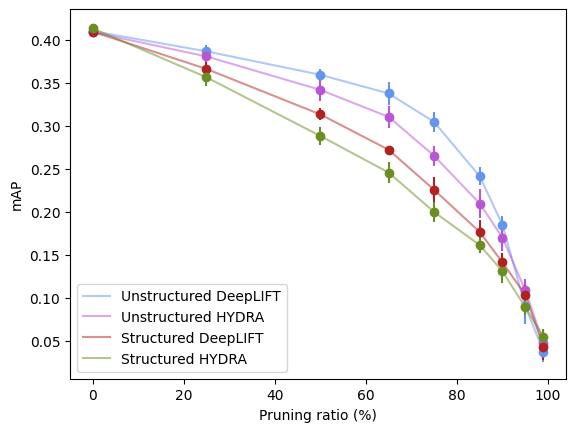
\includegraphics[width=1\linewidth]{figures/mAP1.PNG}
      \caption{mAP}
      \label{fig:mAP1}
    \end{subfigure}%
    \begin{subfigure}[b]{.5\textwidth}
      \centering
      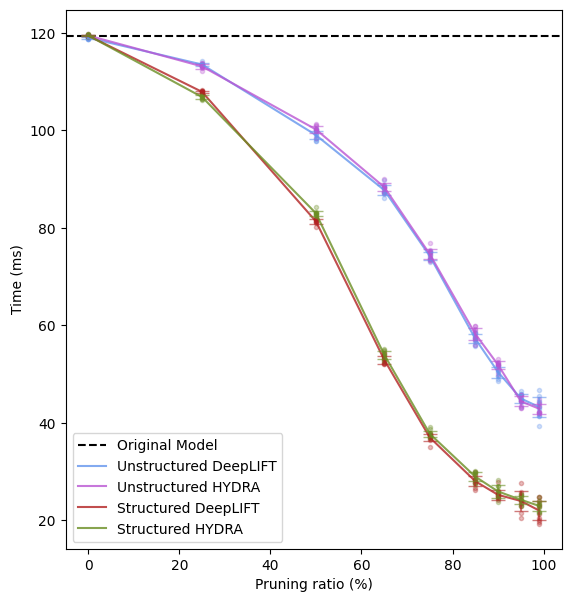
\includegraphics[width=1\linewidth]{figures/time1.PNG}
      \caption{Inference time}
      \label{fig:time1}
    \end{subfigure}
    \caption{Comparison of DeepLIFT versus HYDRA initialized models with both unstructured and structured pruning, through different pruning ratios}
    \label{fig:result1}
\end{figure}

\begin{table}[htbp]
    \caption{p-values from ANOVA tests on mAP}
    \begin{center}
    \begin{tabular}{ |p{3cm}|p{1.2cm}|p{1.2cm}|p{1.2cm}|p{1.2cm}|p{1.2cm}|p{1.2cm}|p{1.2cm}|p{1.2cm}|p{1.2cm}|  }
     \hline
     Pruning ratio  & 0\% & 25\%& 50\%& 65\%& 75\%& 85\%& 90\%& 95\%& 99\%\\
     \hline
     DeepLIFT vs. HYDRA (Unstructured)    & 1.03e-01& 9.53e-02& 1.71e-03& 3.60e-04& 1.57e-06& 1.64e-04& 2.43e-02& 3.54e-02& 1.86e-01 \\
     DeepLIFT vs. HYDRA (Structured)     & 1.48e-02& 3.60e-02& 1.18e-05& 1.24e-05& 6.91e-04& 1.17e-02& 8.99e-02& 8.87e-03& 5.80e-02\\
     \hline
     Unstructured vs. Structured (DeepLIFT)      & 6.52e-01& 2.35e-05& 3.70e-11& 4.25e-11&4.20e-10& 1.13e-09& 5.46e-08& 1.09e-01&3.99e-01 \\
     Unstructured vs. Structured (HYDRA)    & 9.00e-04& 1.11e-05& 1.17e-08& 3.05e-09&4.44e-10& 6.27e-07& 1.80e-05& 1.83e-03&2.42e-01\\
    %  \hline
    %  Greyscale       & 1.13e-23& 1.74e-15& 1.06e-13& 1.18e-11& 2.53e-12& 2.77e-& 1.75e-05& 9.25e-02& 5.06e-01 \\
     \hline
    \end{tabular}
    \end{center}
    \label{tab:p-mAP}
\end{table}

\begin{table}[htbp]
    \caption{p-values from ANOVA tests on inference time}
    \begin{center}
    \begin{tabular}{ |p{3cm}|p{1.2cm}|p{1.2cm}|p{1.2cm}|p{1.2cm}|p{1.2cm}|p{1.2cm}|p{1.2cm}|p{1.2cm}|p{1.2cm}|  }
     \hline
     Pruning ratio  & 0\% & 25\%& 50\%& 65\%& 75\%& 85\%& 90\%& 95\%& 99\%\\
     \hline
     DeepLIFT vs. HYDRA (Unstructured)    & 1.28e-05& 5.61e-02& 7.16e-03& 1.44e-01& 3.96e-01& 7.69e-02& 4.37e-03& 2.05e-01& 6.64e-01 \\
     DeepLIFT vs. HYDRA (Structured)     & 5.13e-01& 1.81e-06& 2.80e-06& 1.37e-02& 4.21e-02& 6.36e-02& 2.06e-01& 7.33e-01& 2.15e-01\\
     \hline
     Unstructured vs. Structured (DeepLIFT)      & 1.75e-04& 4.13e-19& 4.31e-21& 1.07e-24& 2.76e-26& 2.02e-22& 6.17e-21& 1.85e-16& 1.68e-14 \\
     Unstructured vs. Structured (HYDRA)    & 8.70e-01& 2.76e-17& 1.03e-21& 8.97e-26& 3.45e-25& 1.30e-21& 3.55e-21& 2.36e-20& 1.56e-19\\
    %  \hline
    %  Greyscale       & 6.11e-09& 2.07e-07& 1.14e-05& 4.42e-04& 2.08e-01& 5.59e-01& 2.62e-01& 3.98e-02& 4.82e-01 \\
     \hline
    \end{tabular}
    \end{center}
    \label{tab:p-time}
\end{table}


% deeplift better
When comparing the mAP performance between models pruned using DeepLIFT initialization versus scaled initialization in Fig. \ref{fig:mAP1}, DeepLIFT consistently outperforms scaled initialization within the 50\%-85\% pruning ratio range for both pruning methods. This superiority is statistically validated by one-way ANOVA tests, all of which yield p-values below the 0.05 significance threshold, as detailed in Table \ref{tab:p-mAP}. Using DeepLIFT to set importance scores for pruning can be more effective than scaled initialization because DeepLIFT directly calculates the contribution of each weight or neuron to the final output, rather than relying solely on the magnitude of the weights. In scaled initialization, importance is often inferred from the size or magnitude of weights, assuming larger weights contribute more to the model’s performance. 

However, this approach doesn’t account for the complex, non-linear relationships between weights and the model's predictions. Large weights might not always be crucial to the output, especially if they are part of redundant or less influential paths in the network. DeepLIFT, on the other hand, provides an attribution score for each weight by measuring its actual impact on the model’s output relative to a reference state. This attribution-based approach is more precise, as it captures how each weight contributes to the final prediction, rather than just its size. 

By focusing on weights that genuinely affect the model’s decisions, DeepLIFT can help retain the most functionally important components of the network during pruning, leading to a more efficient model that maintains higher performance even with fewer parameters. This tailored pruning is particularly valuable in complex tasks like object detection, where specific features and spatial relationships are critical for accurate predictions.

% compare time
When comparing the inference time between pruned models using the two different initialization methods in Fig. \ref{fig:time1}, there is not a clear difference between the methods with both unstructured and structured pruning. Regardless of the initial scoring method, the pruning algorithm aims to reduce the network to achieve a target pruning rate, resulting in a final model whose inference efficiency depends primarily on its size and structure rather than on the specific initial importance scores. The p-values from ANOVA tests in Table \ref{tab:p-time} mostly support the observation, with most of them above 0.05. However, DeepLift initialization does show small improvements over scaled initialization at 50\% pruning ratio for both pruning methods. 

% init time penalty
Lastly, when using the DeepLIFT initialization method over HYDRA's scaled initialization, there is an increase in the time taken to initialize the importance scores. Scaled initialization needs on average 18 seconds, however DeepLIFT requires almost triple the time at 49 seconds on average. There may be several reasons why DeepLIFT takes longer to run compared to scaled initialization. First, DeepLIFT’s reliance on reference-based computations involves calculating the difference between each neuron’s activation and a chosen baseline or reference state, which is a more involved process than simply using the magnitude of the neurons' weights. This difference-from-reference approach allows DeepLIFT to propagate importance scores accurately, even when gradients are zero, but it adds an additional layer of computation. Additionally, DeepLIFT’s optional rules, like RevealCancel, require separate treatment of positive and negative contributions at each neuron, which can double the amount of computational effort. This is especially demanding in deep networks with complex interactions, where the RevealCancel rule must carefully handle interdependencies among inputs to ensure correct importance scores. 


\subsection{Unstructured vs Structured Pruning}
\label{sec2}
When evaluating the performance difference between unstructured and structured pruning, Fig. \ref{fig:mAP1} illustrates that unstructured pruning consistently achieves higher mAP than structured pruning across pruning ratios ranging from 25\% to 90\% for both initialization methods. This finding is further supported by the p-values from the ANOVA tests presented in Table \ref{tab:p-mAP}. Structured pruning generally results in lower mAP compared to unstructured pruning because it removes entire filters, channels, or even layers, which directly impacts the model’s architecture and reduces its ability to capture fine-grained information. By removing whole structures, such as convolutional filters, structured pruning creates gaps in the model’s feature extraction capabilities, leading to a less detailed representation of the input. This is particularly detrimental to object detection tasks that rely on capturing diverse features across multiple scales and locations. As a result, structured pruning often has a more pronounced negative effect on mAP, as the model’s capacity to accurately locate and classify objects diminishes.

While the initialization method did not have a significant effect on the inference time performance, Fig. \ref{fig:time1} shows a significant difference between the two pruning methods. As the pruning rate increases, there is an increasing gap in the time needed for the pruned models to evaluate an image. Starting from 65\% pruning ratio, structured pruned models require only approximately half the time compared to unstructured pruned models at the same pruning ratio. The one-way ANOVA tests confirm these observations in Table \ref{tab:p-time}. Structured pruning excels in improving inference time because it results in a more regularized and optimized network architecture. Unlike unstructured pruning, which removes individual weights sparsely throughout the network, structured pruning produces a model with fewer filters or layers but with a consistent structure that is easier for hardware like GPUs to process. This regularity allows for better memory access patterns and more efficient use of processing resources, leading to faster computations during inference. Consequently, while structured pruning may sacrifice some accuracy in mAP, it provides a significant boost in inference speed, making it a practical choice for applications requiring real-time performance.

\subsection{Effect of Greyscale on Performance}
\label{sec3}
\begin{figure}
    \centering
    \captionsetup{justification=centering}
    \begin{subfigure}[b]{.5\textwidth}
      \centering
      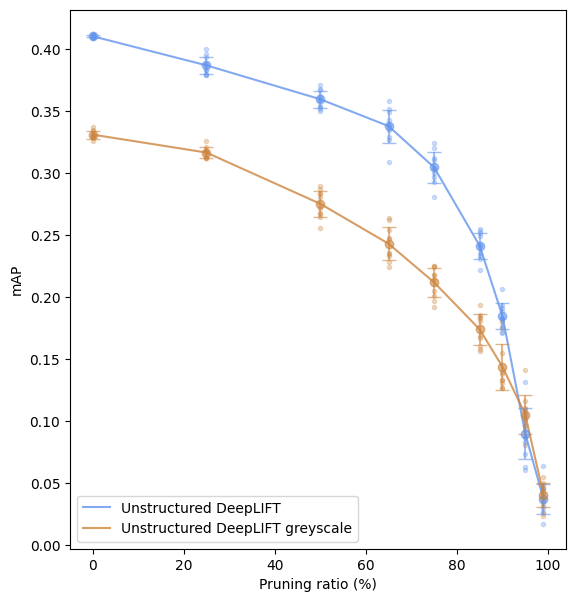
\includegraphics[width=1\linewidth]{figures/mAP2.PNG}
      \caption{mAP}
      \label{fig:mAP2}
    \end{subfigure}%
    \begin{subfigure}[b]{.5\textwidth}
      \centering
      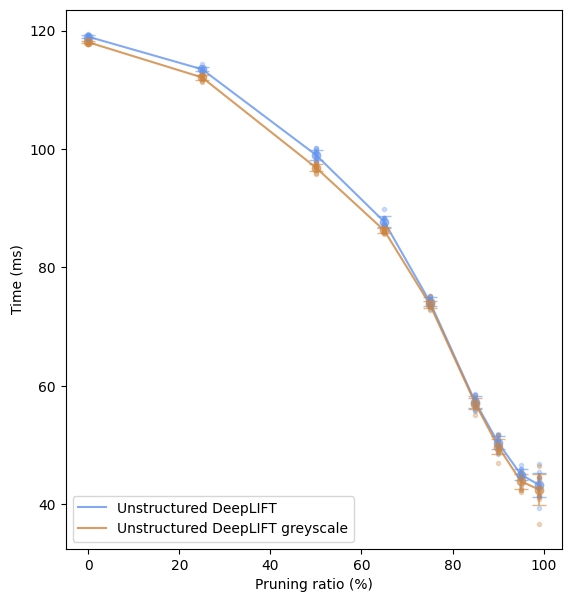
\includegraphics[width=1\linewidth]{figures/time2.PNG}
      \caption{Inference time}
      \label{fig:time2}
    \end{subfigure}
    \caption{Comparison of performance between colour and greyscale images on unstructured pruned models initialized with DeepLIFT}
    \label{fig:result2}
\end{figure}

\begin{table}[htbp]
    \caption{p-values from ANOVA tests on mAP}
    \begin{center}
    \begin{tabular}{ |p{3.3cm}|p{1.2cm}|p{1.2cm}|p{1.2cm}|p{1.2cm}|p{1.2cm}|p{1.2cm}|p{1.2cm}|p{1.2cm}|p{1.2cm}|  }
    \hline
    Pruning ratio  & 0\% & 25\%& 50\%& 65\%& 75\%& 85\%& 90\%& 95\%& 99\%\\
     \hline
     Greyscale vs Colour (Unstructured DeepLIFT)      & 1.13e-23& 1.74e-15& 1.06e-13& 1.18e-11& 2.53e-12& 2.77e-10& 1.75e-05& 9.25e-02& 5.06e-01 \\
     \hline
    \end{tabular}
    \end{center}
    \label{tab:p2-mAP}
\end{table}

\begin{table}[htbp]
    \caption{p-values from ANOVA tests on inference time}
    \begin{center}
    \begin{tabular}{ |p{3.3cm}|p{1.2cm}|p{1.2cm}|p{1.2cm}|p{1.2cm}|p{1.2cm}|p{1.2cm}|p{1.2cm}|p{1.2cm}|p{1.2cm}|  }
     \hline
     Pruning ratio  & 0\% & 25\%& 50\%& 65\%& 75\%& 85\%& 90\%& 95\%& 99\%\\
     \hline
     Greyscale vs Colour (Unstructured DeepLIFT)       & 6.11e-09& 2.07e-07& 1.14e-05& 4.42e-04& 2.08e-01& 5.59e-01& 2.62e-01& 3.98e-02& 4.82e-01 \\
     \hline
    \end{tabular}
    \end{center}
    \label{tab:p2-time}
\end{table}


We evaluated the performance of the pruning pipeline with greyscale images. The training images are identical to those used in previous experiments but are converted to greyscale following the Rec. 601 Standard. This conversion employs a weighted average with standardized weights of 0.299 for red, 0.587 for green, and 0.114 for blue channels to account for human eye sensitivity. The resulting greyscale images were then replicated across all three channels to match the input shape required by the YOLOv3 model. For this experiment, we utilized the unstructured DeepLIFT variant of the pruning pipeline, as it demonstrated the highest mAP performance in earlier tests.

In the mAP performance shown in Fig. \ref{fig:mAP2}, models trained with greyscale images exhibit significantly lower mAP compared to those trained with colored images, particularly at lower pruning ratios ranging from 0\% to 65\%. However, as the pruning ratio increases, the performance gap narrows, and by 95\% and 99\% pruning ratios, the presence or absence of color no longer impacts model performance. These findings are corroborated by the ANOVA test p-values presented in Table \ref{tab:p2-mAP}.

The observed performance gap between models trained on greyscale versus coloured images can be explained by the reduced information available in greyscale images. Object detection models, particularly those like YOLOv3, leverage colour information to help distinguish objects from the background and from each other, as well as to capture subtle variations in texture, lighting, and shading that contribute to accurate object localization and classification. In coloured images, the model can use the distinct red, green, and blue channels to capture these variations, which aids in creating a more detailed and nuanced feature representation of each object. 

In contrast, greyscale images provide only intensity information, limiting the model's ability to distinguish certain objects based on colour-related features, and this can negatively impact mAP performance, particularly at lower pruning ratios where the network retains more parameters and thus has a greater capacity to process detailed information. For example, without colour information, it becomes challenging for the model to distinguish between objects like lemons and limes, as both share similar shapes and textures; the absence of yellow or green colour cues can lead to confusion in classification.

At lower pruning ratios (0\% to 65\%), where more network parameters are retained, the colour information plays a significant role in enhancing model performance, as the model can make full use of colour-based features. The lack of colour in greyscale images leads to a noticeable drop in mAP at these pruning rates because the model has fewer cues to differentiate objects and backgrounds, resulting in less precise detection. As the pruning ratio increases, however, the network becomes increasingly constrained, losing a substantial amount of capacity to capture and process intricate features, including those related to colour. 

At higher pruning rates (95\% and 99\%), both greyscale and colour-based models are similarly limited in their feature extraction abilities due to the severe reduction in parameters. This means that even in the colour-based model, the remaining network capacity is not sufficient to utilize the colour information effectively, leading to a convergence in performance between the greyscale and colour models. Essentially, at extreme pruning levels, the model's ability to leverage additional colour information diminishes, resulting in similar mAP performance for both greyscale and colour inputs.

% time
When considering the inference time performance, it can be observed from Fig. \ref{fig:time2} that the greyscale-trained models are slightly faster at evaluating images at smaller pruning ratios below 65\% pruning ratio. This slight improvement in inference speed can be attributed to the simpler feature extraction process involved when working with greyscale images. Since greyscale images lack colour information, the model processes fewer distinct features per image, requiring less computation to analyze intensity-only patterns compared to the more complex, multi-channel colour features. In colour images, the model needs to process three channels, each containing unique information that must be integrated to capture subtle differences in texture, colour gradients, and object boundaries. As the pruning ratio increases, the network's capacity to process any detailed information—whether from colour or greyscale—declines sharply. This reduction in complexity due to aggressive pruning diminishes the initial speed advantage observed with greyscale inputs. By the time the pruning ratio exceeds 65\%, both greyscale and colour-trained models are similarly limited in their feature extraction abilities, leading to convergence in inference time performance. p-values in Table \ref{tab:p2-time} show that there is no statistical difference between the two configurations higher than 75\% pruning ratio.

\subsection{Sample Images}

\begin{figure}
    \centering
    \captionsetup{justification=centering}
    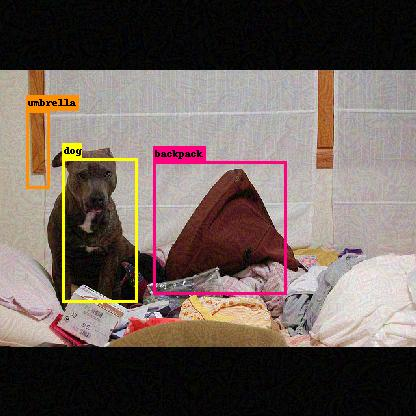
\includegraphics[width=0.6\linewidth]{figures/attack_after_22192.jpg}
    \caption{COCO image 22192 results from models pruned with different initialization, structure, and ratio}
    \label{fig:temp}
\end{figure}

\section{Conclusion}

In conclusion, this study successfully adapted the HYDRA pruning framework to enhance both efficiency and robustness in object detection by implementing structured and unstructured pruning strategies on the YOLOv3 model. Through a comprehensive evaluation across different pruning levels, it was observed that unstructured pruning consistently outperformed structured pruning in maintaining higher mean Average Precision (mAP), particularly at moderate pruning ratios, which is crucial for retaining detection accuracy in complex environments. By leveraging DeepLIFT for importance scoring, the pruning process was made more precise, targeting weights with minimal contribution to the output. This refinement in importance scoring allowed for more efficient pruning without compromising the network's capacity to detect and localize objects accurately, making it suitable for applications that demand both speed and high performance, such as autonomous driving or real-time surveillance. Moreover, the integration of robust training objectives within the HYDRA framework provided resilience against adversarial attacks, enabling the pruned model to maintain robust accuracy even under adversarial conditions.

For future work, several directions could further enhance robust object detection. First, exploring hybrid pruning techniques that combine the advantages of both structured and unstructured pruning might lead to more optimal trade-offs between performance and efficiency. Additionally, testing this pruning framework on other object detection models, such as Faster R-CNN or SSD, could provide insights into its generalizability across architectures. Another potential avenue is to refine robust training objectives further to better withstand a broader range of adversarial attacks, potentially integrating new defensive strategies that adapt dynamically based on attack characteristics. Lastly, extending this framework to multi-modal inputs, such as video data, could expand its applicability to areas like surveillance and autonomous driving, where real-time and robust object detection is critical.



% if have a single appendix:
%\appendix[Proof of the Zonklar Equations]
% or
%\appendix  % for no appendix heading
% do not use \section anymore after \appendix, only \section*
% is possibly needed

% use appendices with more than one appendix
% then use \section to start each appendix
% you must declare a \section before using any
% \subsection or using \label (\appendices by itself
% starts a section numbered zero.)
%

\newpage
\printbibliography
\newpage

\appendices
\section{Raw experiment data}
\label{appendix:tables}

\begin{table}[htbp]
    \caption{Unstructured DeepLIFT mAP}
    \begin{center}
    \begin{tabular}{ |p{2cm}|p{1cm}|p{1cm}|p{1cm}|p{1cm}|p{1cm}|p{1cm}|p{1cm}|p{1cm}|p{1cm}|  }
     \hline
     Pruning ratio  & 0\% & 25\%& 50\%& 65\%& 75\%& 85\%& 90\%& 95\%& 99\%\\
     \hline
        run 1 & 0.410& 0.380& 0.353& 0.358& 0.293& 0.249& 0.176& 0.103& 0.046\\
        run 2 & 0.411& 0.379& 0.368& 0.343& 0.311& 0.242& 0.172& 0.097& 0.036\\
        run 3 & 0.410& 0.387& 0.360& 0.335& 0.300& 0.231& 0.189& 0.093& 0.045\\
        run 4 & 0.411& 0.383& 0.352& 0.327& 0.304& 0.253& 0.191& 0.087& 0.030\\
        run 5 & 0.409& 0.379& 0.371& 0.349& 0.312& 0.241& 0.183& 0.083& 0.039\\
        run 6 & 0.410& 0.396& 0.350& 0.339& 0.281& 0.222& 0.194& 0.074& 0.017\\
        run 7 & 0.412& 0.400& 0.354& 0.352& 0.297& 0.252& 0.183& 0.063& 0.064\\
        run 8 & 0.410& 0.394& 0.367& 0.329& 0.304& 0.236& 0.182& 0.108& 0.027\\
        run 9 & 0.411& 0.388& 0.362& 0.338& 0.324& 0.233& 0.171& 0.061& 0.032\\
        run 10 & 0.410& 0.383& 0.359& 0.309& 0.320& 0.255& 0.207& 0.132& 0.037\\
     \hline
        max     & 0.412 &0.400 &  0.371& 0.358 &0.324& 0.255 &0.207 &0.132& 0.064\\
        min     & 0.409 &0.379 &0.350 & 0.309 &0.281& 0.222 &0.171 &0.061& 0.017\\
        avg     & 0.410 &0.386 &0.359& 0.337& 0.304 &0.241 &0.184& 0.090 &0.037\\
        std dev & 8.0e-04 &7.1e-03 &6.9e-03& 1.3e-02 &1.2e-02& 1.0e-02& 1.0e-02& 2.0e-02 &1.2e-02\\
     \hline
    \end{tabular}
    \end{center}
    \label{tab:a1}
\end{table}

\begin{table}[htbp]
    \caption{Unstructured HYDRA mAP}
    \begin{center}
    \begin{tabular}{ |p{2cm}|p{1cm}|p{1cm}|p{1cm}|p{1cm}|p{1cm}|p{1cm}|p{1cm}|p{1cm}|p{1cm}|  }
     \hline
     Pruning ratio  & 0\% & 25\%& 50\%& 65\%& 75\%& 85\%& 90\%& 95\%& 99\%\\
     \hline
        run 1&0.411&0.379&0.342&0.334&0.279&0.187&0.175&0.101&0.062\\
        run 2&0.407&0.366&0.328&0.310&0.266&0.218&0.192&0.114&0.055\\
        run 3&0.410&0.382&0.323&0.327&0.258&0.235&0.190&0.122&0.047\\
        run 4&0.409&0.390&0.335&0.300&0.256&0.197&0.150&0.120&0.029\\
        run 5&0.411&0.379&0.356&0.313&0.267&0.214&0.158&0.098&0.052\\
        run 6&0.408&0.382&0.342&0.290&0.237&0.228&0.157&0.096&0.041\\
        run 7&0.407&0.380&0.328&0.294&0.275&0.220&0.172&0.136&0.030\\
        run 8&0.409&0.374&0.360&0.317&0.274&0.182&0.188&0.099&0.016\\
        run 9&0.413&0.391&0.355&0.307&0.274&0.195&0.161&0.110&0.073\\
        run 10&0.407&0.387&0.351&0.314&0.266&0.221&0.156&0.091&0.063\\
     \hline
        max     &0.413&0.391&0.360&0.334&0.279&0.235&0.192&0.136&0.073\\
        min     &0.407&0.366&0.323&0.290&0.237&0.182&0.150&0.091&0.016\\
        avg     &0.409&0.381&0.342&0.311&0.265&0.210&0.170&0.109&0.047\\
        std dev &1.9e-03&7.1e-03&1.3e-02&1.3e-02&1.2e-02&1.7e-02&1.5e-02&1.3e-02&1.7e-02\\
     \hline
    \end{tabular}
    \end{center}
    \label{tab:a2}
\end{table}

\begin{table}[htbp]
    \caption{Structured DeepLIFT mAP}
    \begin{center}
    \begin{tabular}{ |p{2cm}|p{1cm}|p{1cm}|p{1cm}|p{1cm}|p{1cm}|p{1cm}|p{1cm}|p{1cm}|p{1cm}|  }
     \hline
     Pruning ratio  & 0\% & 25\%& 50\%& 65\%& 75\%& 85\%& 90\%& 95\%& 99\%\\
     \hline
     run 1&0.409&0.375&0.311&0.269&0.220&0.199&0.139&0.098&0.048\\
     run 2&0.411&0.369&0.312&0.268&0.218&0.182&0.126&0.103&0.040\\
     run 3&0.407&0.353&0.313&0.275&0.232&0.150&0.139&0.081&0.062\\
     run 4&0.410&0.360&0.318&0.269&0.214&0.167&0.149&0.102&0.039\\
     run 5&0.411&0.361&0.303&0.278&0.230&0.177&0.142&0.108&0.052\\
     run 6&0.411&0.363&0.304&0.275&0.211&0.165&0.141&0.101&0.011\\
     run 7&0.406&0.376&0.323&0.273&0.204&0.180&0.152&0.119&0.024\\
     run 8&0.408&0.381&0.322&0.274&0.228&0.168&0.142&0.110&0.053\\
     run 9&0.418&0.361&0.321&0.264&0.239&0.190&0.159&0.121&0.058\\
     run 10&0.408&0.365&0.308&0.278&0.260&0.187&0.122&0.090&0.041\\
     \hline
        max     &0.418&0.381&0.323&0.278&0.260&0.199&0.159&0.121&0.062\\
        min     &0.406&0.353&0.303&0.264&0.204&0.150&0.122&0.081&0.011\\
        avg     &0.410&0.366&0.314&0.272&0.226&0.176&0.141&0.103&0.043\\
        std dev &3.2e-03&8.2e-03&6.9e-03&4.4e-03&1.5e-02&1.4e-02&1.1e-02&1.2e-02&1.5e-02\\
     \hline
    \end{tabular}
    \end{center}
    \label{tab:a3}
\end{table}

\begin{table}[htbp]
    \caption{Structured HYDRA mAP}
    \begin{center}
    \begin{tabular}{ |p{2cm}|p{1cm}|p{1cm}|p{1cm}|p{1cm}|p{1cm}|p{1cm}|p{1cm}|p{1cm}|p{1cm}|  }
     \hline
     Pruning ratio  & 0\% & 25\%& 50\%& 65\%& 75\%& 85\%& 90\%& 95\%& 99\%\\
     \hline
     run 1&0.413&0.352&0.271&0.264&0.204&0.163&0.120&0.102&0.054\\
     run 2&0.410&0.364&0.309&0.223&0.194&0.160&0.115&0.079&0.058\\
     run 3&0.413&0.367&0.291&0.239&0.195&0.155&0.147&0.081&0.065\\
     run 4&0.411&0.348&0.297&0.243&0.186&0.168&0.142&0.087&0.057\\
     run 5&0.411&0.349&0.280&0.260&0.188&0.160&0.129&0.091&0.061\\
     run 6&0.415&0.368&0.282&0.238&0.225&0.172&0.143&0.085&0.053\\
     run 7&0.420&0.339&0.287&0.246&0.191&0.176&0.129&0.084&0.036\\
     run 8&0.413&0.370&0.300&0.255&0.209&0.147&0.137&0.079&0.040\\
     run 9&0.416&0.359&0.285&0.232&0.199&0.164&0.102&0.105&0.059\\
     run 10&0.415&0.351&0.282&0.258&0.207&0.148&0.143&0.097&0.062\\
     \hline
        max     &0.420&0.370&0.309&0.264&0.225&0.176&0.147&0.105&0.065\\
        min     &0.410&0.339&0.271&0.223&0.186&0.147&0.102&0.079&0.036\\
        avg     &0.414&0.357&0.288&0.246&0.200&0.161&0.131&0.089&0.054\\
        std dev &2.8e-03&9.9e-03&1.1e-02&1.3e-02&1.1e-02&9.0e-03&1.4e-02&9.0e-03&9.0e-03\\
     \hline
    \end{tabular}
    \end{center}
    \label{tab:a4}
\end{table}

\begin{table}[htbp]
    \caption{Unstructured DeepLIFT Greyscale mAP}
    \begin{center}
    \begin{tabular}{ |p{2cm}|p{1cm}|p{1cm}|p{1cm}|p{1cm}|p{1cm}|p{1cm}|p{1cm}|p{1cm}|p{1cm}|  }
     \hline
     Pruning ratio  & 0\% & 25\%& 50\%& 65\%& 75\%& 85\%& 90\%& 95\%& 99\%\\
     \hline
     run 1&0.329&0.312&0.281&0.236&0.201&0.194&0.175&0.087&0.034\\
     run 2&0.328&0.318&0.287&0.247&0.192&0.158&0.127&0.096&0.049\\
     run 3&0.331&0.321&0.272&0.228&0.218&0.161&0.138&0.110&0.050\\
     run 4&0.326&0.317&0.256&0.254&0.225&0.157&0.131&0.101&0.026\\
     run 5&0.331&0.313&0.267&0.233&0.218&0.181&0.180&0.105&0.044\\
     run 6&0.337&0.326&0.283&0.264&0.205&0.186&0.133&0.106&0.055\\
     run 7&0.330&0.319&0.265&0.224&0.224&0.184&0.155&0.111&0.038\\
     run 8&0.334&0.312&0.290&0.248&0.197&0.183&0.140&0.141&0.046\\
     run 9&0.330&0.316&0.284&0.262&0.214&0.169&0.133&0.116&0.042\\
     run 10&0.335&0.312&0.268&0.235&0.225&0.167&0.127&0.081&0.024\\
     \hline
        max     &0.337&0.326&0.290&0.264&0.225&0.194&0.180&0.141&0.055\\
        min     &0.326&0.312&0.256&0.224&0.192&0.157&0.127&0.081&0.024\\
        avg     &0.331&0.317&0.275&0.243&0.212&0.174&0.144&0.105&0.041\\
        std dev &3.2e-03&4.4e-03&1.1e-02&1.3e-02&1.2e-02&1.2e-02&1.8e-02&1.6e-02&9.7e-03\\
     \hline
    \end{tabular}
    \end{center}
    \label{tab:a5}
\end{table}

\begin{table}[htbp]
    \caption{Unstructured DeepLIFT Time}
    \begin{center}
    \begin{tabular}{ |p{2cm}|p{1cm}|p{1cm}|p{1cm}|p{1cm}|p{1cm}|p{1cm}|p{1cm}|p{1cm}|p{1cm}|  }
     \hline
     Pruning ratio  & 0\% & 25\%& 50\%& 65\%& 75\%& 85\%& 90\%& 95\%& 99\%\\
     \hline
        run 1&118.8&113.6&98.4&87.6&73.3&55.9&49.5&44.8&45.4\\
        run 2&119.4&113.6&100.2&88.3&73.7&55.8&49.0&44.7&41.4\\
        run 3&119.1&113.3&99.2&87.4&74.5&56.9&50.7&45.0&39.3\\
        run 4&118.9&113.3&98.2&89.8&75.2&57.1&49.7&44.6&42.9\\
        run 5&118.7&113.4&100.2&87.1&73.8&57.3&51.7&44.4&46.8\\
        run 6&118.7&113.3&99.8&87.0&75.2&56.5&50.4&44.6&43.3\\
        run 7&119.2&114.3&97.8&87.3&74.7&58.6&51.8&45.9&44.5\\
        run 8&119.1&113.1&99.0&88.3&73.7&58.4&50.9&46.6&43.2\\
        run 9&119.1&113.3&99.5&88.3&75.0&57.4&51.7&43.3&41.3\\
        run 10&118.8&113.6&97.8&86.1&72.9&58.4&48.5&46.0&44.3\\
     \hline
        max     &119.4&114.3&100.2&89.8&75.2&58.6&51.8&46.6&46.8\\
        min     &118.7&113.1&97.8&86.1&72.9&55.8&48.5&43.3&39.3\\
        avg     &119.0&113.5&99.0&87.7&74.2&57.2&50.4&45.0&43.2\\
        std dev &2.2e-01&3.2e-01&8.8e-01&9.6e-01&7.8e-01&9.6e-01&1.1e+00&9.0e-01&2.1e+00\\
     \hline
    \end{tabular}
    \end{center}
    \label{tab:a6}
\end{table}

\begin{table}[htbp]
    \caption{Unstructured HYDRA Time}
    \begin{center}
    \begin{tabular}{ |p{2cm}|p{1cm}|p{1cm}|p{1cm}|p{1cm}|p{1cm}|p{1cm}|p{1cm}|p{1cm}|p{1cm}|  }
     \hline
     Pruning ratio  & 0\% & 25\%& 50\%& 65\%& 75\%& 85\%& 90\%& 95\%& 99\%\\
     \hline
     run 1&119.5&113.1&100.8&88.1&75.0&59.8&50.0&45.7&44.1\\
     run 2&119.4&113.7&99.9&87.2&75.4&59.2&52.1&44.4&44.9\\
     run 3&119.4&113.1&99.8&88.1&74.4&57.7&52.5&44.4&41.9\\
     run 4&119.3&113.8&100.1&88.4&75.0&59.1&53.1&45.8&43.9\\
     run 5&119.5&112.8&100.2&88.8&73.1&56.9&52.2&44.4&42.0\\
     run 6&119.4&112.9&101.2&88.2&73.4&57.3&51.9&44.3&42.2\\
     run 7&119.4&112.9&100.3&88.7&74.8&57.9&51.8&43.0&42.0\\
     run 8&119.5&113.4&101.1&88.6&73.7&55.9&51.9&43.0&42.3\\
     run 9&119.5&113.2&98.5&90.0&76.9&58.4&52.2&43.4&42.3\\
     run 10&119.5&112.1&99.8&87.3&74.1&59.9&51.1&45.6&43.4\\
     \hline
        max     &119.5&113.8&101.2&90.0&76.9&59.9&53.1&45.8&44.9\\
        min     &119.3&112.1&98.5&87.2&73.1&55.9&50.0&43.0&41.9\\
        avg     &119.4&113.1&100.2&88.3&74.6&58.2&51.9&44.4&42.9\\
        std dev &6.6e-02&4.6e-01&7.4e-01&7.5e-01&1.1e+00&1.2e+00&7.9e-01&1.0e+00&1.0e+00\\
     \hline
    \end{tabular}
    \end{center}
    \label{tab:a7}
\end{table}

\begin{table}[htbp]
    \caption{Structured DeepLIFT Time}
    \begin{center}
    \begin{tabular}{ |p{2cm}|p{1cm}|p{1cm}|p{1cm}|p{1cm}|p{1cm}|p{1cm}|p{1cm}|p{1cm}|p{1cm}|  }
     \hline
     Pruning ratio  & 0\% & 25\%& 50\%& 65\%& 75\%& 85\%& 90\%& 95\%& 99\%\\
     \hline
     run 1&119.4&108.2&81.2&54.4&35.1&26.7&24.9&24.1&20.1\\
     run 2&119.3&108.0&80.9&53.0&37.1&28.0&25.5&20.4&20.5\\
     run 3&119.3&107.9&81.3&52.3&38.0&29.2&24.5&25.9&23.9\\
     run 4&119.2&108.1&81.9&53.1&37.2&30.0&24.1&27.6&19.7\\
     run 5&119.7&107.4&80.1&52.1&36.6&26.2&25.6&25.3&23.2\\
     run 6&119.3&107.8&81.7&52.2&37.4&28.3&24.6&23.4&24.7\\
     run 7&119.3&108.1&81.4&52.7&37.5&27.6&24.9&23.6&24.7\\
     run 8&119.4&107.8&81.1&53.0&36.4&27.9&25.0&21.4&22.9\\
     run 9&119.5&107.4&81.8&54.4&37.0&27.7&27.8&23.0&21.2\\
     run 10&119.6&108.1&81.8&52.1&37.6&28.5&25.3&25.0&19.2\\
     \hline
        max     &119.7&108.2&81.9&54.4&38.0&30.0&27.8&27.6&24.7\\
        min     &119.2&107.4&80.1&52.1&35.1&26.2&24.1&20.4&19.2\\
        avg     &119.4&107.9&81.3&52.9&37.0&28.0&25.2&24.0&22.0\\
        std dev &1.5e-01&2.7e-01&5.2e-01&8.2e-01&7.7e-01&1.0e+00&9.6e-01&2.0e+00&2.0e+00\\
     \hline
    \end{tabular}
    \end{center}
    \label{tab:a8}
\end{table}

\begin{table}[htbp]
    \caption{Structured HYDRA Time}
    \begin{center}
    \begin{tabular}{ |p{2cm}|p{1cm}|p{1cm}|p{1cm}|p{1cm}|p{1cm}|p{1cm}|p{1cm}|p{1cm}|p{1cm}|  }
     \hline
     Pruning ratio  & 0\% & 25\%& 50\%& 65\%& 75\%& 85\%& 90\%& 95\%& 99\%\\
     \hline
     run 1&119.5&107.2&84.3&53.9&39.1&28.3&23.8&24.1&23.2\\
     run 2&119.7&106.4&83.1&54.7&37.9&30.1&27.0&23.7&23.9\\
     run 3&119.3&106.5&83.0&53.7&37.0&27.3&26.1&23.0&22.8\\
     run 4&119.4&107.2&82.9&53.0&37.9&29.9&27.0&24.2&21.8\\
     run 5&119.3&106.6&82.6&53.5&37.4&29.9&26.0&25.0&23.6\\
     run 6&119.2&106.2&83.0&54.2&37.6&29.5&24.5&22.9&24.7\\
     run 7&119.6&107.4&82.9&54.9&38.7&28.3&28.3&25.3&23.4\\
     run 8&119.3&106.9&82.5&53.9&37.1&28.9&25.2&24.7&21.6\\
     run 9&119.7&106.8&82.2&55.2&36.9&27.6&26.0&25.1&21.8\\
     run 10&119.5&107.0&83.3&52.6&37.8&29.7&25.2&24.2&22.8\\
     \hline
        max     &119.7&107.4&84.3&55.2&39.1&30.1&28.3&25.3&24.7\\
        min     &119.2&106.2&82.2&52.6&36.9&27.3&23.8&22.9&21.6\\
        avg     &119.5&106.8&83.0&54.0&37.7&28.9&25.9&24.2&23.0\\
        std dev &1.7e-01&3.7e-01&5.3e-01&7.8e-01&6.8e-01&9.7e-01&1.2e+00&7.9e-01&9.6e-01\\
     \hline
    \end{tabular}
    \end{center}
    \label{tab:a9}
\end{table}

\begin{table}[htbp]
    \caption{Unstructured DeepLIFT Greyscale Time}
    \begin{center}
    \begin{tabular}{ |p{2cm}|p{1cm}|p{1cm}|p{1cm}|p{1cm}|p{1cm}|p{1cm}|p{1cm}|p{1cm}|p{1cm}|  }
     \hline
     Pruning ratio  & 0\% & 25\%& 50\%& 65\%& 75\%& 85\%& 90\%& 95\%& 99\%\\
     \hline
     run 1&117.8&112.5&95.8&86.0&73.6&57.8&50.2&42.4&44.5\\
     run 2&118.1&112.0&97.7&86.0&74.6&56.1&48.7&45.1&46.5\\
     run 3&117.9&112.1&97.0&86.6&73.8&55.0&51.1&42.3&42.2\\
     run 4&118.1&111.4&96.4&86.1&72.8&57.9&51.7&45.2&44.6\\
     run 5&117.8&111.8&96.8&85.8&73.4&56.4&48.8&42.1&41.6\\
     run 6&118.2&112.4&97.3&86.4&73.5&57.2&50.6&42.8&42.5\\
     run 7&118.1&112.5&96.0&86.5&73.7&56.8&49.6&45.4&36.6\\
     run 8&118.3&111.5&96.9&87.0&73.6&58.1&49.9&43.9&40.9\\
     run 9&118.1&112.2&97.8&86.4&73.4&57.3&49.8&44.7&41.2\\
     run 10&118.1&112.6&96.9&85.6&75.2&57.1&46.9&44.6&43.9\\
     \hline
        max     &118.3&112.6&97.8&87.0&75.2&58.1&51.7&45.4&46.5\\
        min     &117.8&111.4&95.8&85.6&72.8&55.0&46.9&42.1&36.6\\
        avg     &118.0&112.1&96.9&86.2&73.8&57.0&49.7&43.9&42.4\\
        std dev &1.6e-01&4.0e-01&6.2e-01&4.0e-01&6.4e-01&8.9e-01&1.3e+00&1.3e+00&2.6e+00\\
     \hline
    \end{tabular}
    \end{center}
    \label{tab:a10}
\end{table}

% you can choose not to have a title for an appendix
% if you want by leaving the argument blank
% \section{}
% Appendix two text goes here.


% % use section* for acknowledgment
% \section*{Acknowledgment}


% The authors would like to thank...


% Can use something like this to put references on a page
% by themselves when using endfloat and the captionsoff option.
% \ifCLASSOPTIONcaptionsoff
%   \newpage
% \fi



% trigger a \newpage just before the given reference
% number - used to balance the columns on the last page
% adjust value as needed - may need to be readjusted if
% the document is modified later
%\IEEEtriggeratref{8}
% The "triggered" command can be changed if desired:
%\IEEEtriggercmd{\enlargethispage{-5in}}

% references section

% can use a bibliography generated by BibTeX as a .bbl file
% BibTeX documentation can be easily obtained at:
% http://mirror.ctan.org/biblio/bibtex/contrib/doc/
% The IEEEtran BibTeX style support page is at:
% http://www.michaelshell.org/tex/ieeetran/bibtex/
% argument is your BibTeX string definitions and bibliography database(s)
% \bibliography{IEEEabrv,../bib/paper}
% \printbibliography
%
% <OR> manually copy in the resultant .bbl file
% set second argument of \begin to the number of references
% (used to reserve space for the reference number labels box)
% \begin{thebibliography}{1}

% \bibitem{IEEEhowto:kopka}
% H.~Kopka and P.~W. Daly, \emph{A Guide to \LaTeX}, 3rd~ed.\hskip 1em plus
%   0.5em minus 0.4em\relax Harlow, England: Addison-Wesley, 1999.

% \end{thebibliography}



% that's all folks
\end{document}